\documentclass[a4paper]{article}
\usepackage[utf8]{inputenc}
%\usepackage[a4paper, total={150cm, 250cm}]{geometry}

\usepackage{tikz, sidecap, graphicx, amsmath}
\usetikzlibrary{positioning, shapes}

\usepackage{geometry}
 \geometry{
 a4paper,
 total={150mm,257mm},
 left=30mm,
 top=20mm,
 }



\title{Report week 7}
\author{Bård-Kristian Krohg \\ \texttt{baard.krohg@gmail.com}}


\begin{document}
\maketitle

\section{Point set registration problem}
\begin{itemize}
\item Working on code for refining 3D keypoints.
\item Analyzed different ways of estimating the keypoints.
  \begin{itemize}
  \item Iterativeley, by modelling each keypoint as a node in a graph, and limbs as edges
  \item Analytically, by trying to find a transform for the constrained set of points \emph{M} so they are as close to the observed set of points \emph{S} as possible. (I did not find a transform, since we have too many degrees of freedom.)
  \item Updated code to use Eigen for efficiency and readability
  \end{itemize}
\item Started working on an alignment node for calibrating the kinects. Using pre existing feature extraction and matching methods from PCL. Some of the results found here might be helpful for the above problem.
\end{itemize}

\begin{figure}[h]
  \centering
  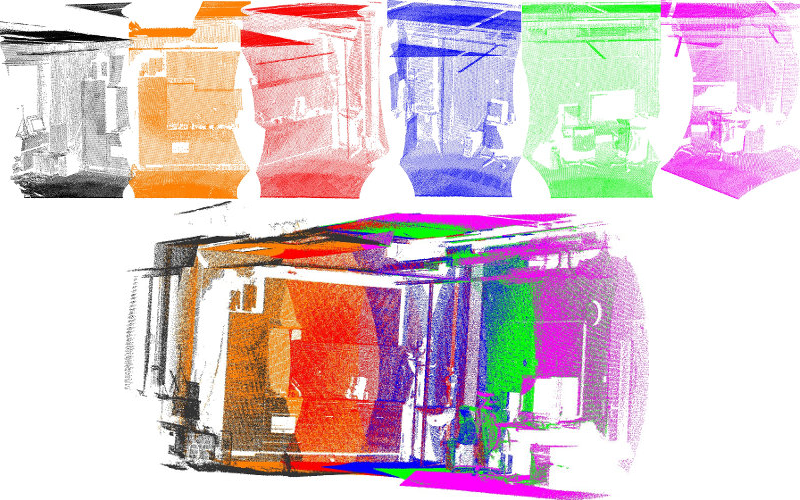
\includegraphics[width=.95\textwidth]{example_iterative_pcl}
  \caption{PCL has many algorithms for aligning point clouds, however, I haven't found a premade method for just getting the transformation directly.}
\end{figure}

\subsection{Next week}
\begin{itemize}
\item Finish point cloud registration, and combine poses from potentially \emph{n} cameras
\end{itemize}
%% \[
%% \begin{bmatrix} a & & \\ & c & \\ & & e\end{bmatrix} \begin{bmatrix} x \\ y \\ z \end{bmatrix} = \begin{bmatrix} 1 \\ 0 \\ 2 \end{bmatrix}
%%       \]
\end{document}

